% Options for packages loaded elsewhere
\PassOptionsToPackage{unicode}{hyperref}
\PassOptionsToPackage{hyphens}{url}
\PassOptionsToPackage{dvipsnames,svgnames,x11names}{xcolor}
%
\documentclass[
  a4paper,
]{scrreport}

\usepackage{amsmath,amssymb}
\usepackage{lmodern}
\usepackage{iftex}
\ifPDFTeX
  \usepackage[T1]{fontenc}
  \usepackage[utf8]{inputenc}
  \usepackage{textcomp} % provide euro and other symbols
\else % if luatex or xetex
  \usepackage{unicode-math}
  \defaultfontfeatures{Scale=MatchLowercase}
  \defaultfontfeatures[\rmfamily]{Ligatures=TeX,Scale=1}
\fi
% Use upquote if available, for straight quotes in verbatim environments
\IfFileExists{upquote.sty}{\usepackage{upquote}}{}
\IfFileExists{microtype.sty}{% use microtype if available
  \usepackage[]{microtype}
  \UseMicrotypeSet[protrusion]{basicmath} % disable protrusion for tt fonts
}{}
\makeatletter
\@ifundefined{KOMAClassName}{% if non-KOMA class
  \IfFileExists{parskip.sty}{%
    \usepackage{parskip}
  }{% else
    \setlength{\parindent}{0pt}
    \setlength{\parskip}{6pt plus 2pt minus 1pt}}
}{% if KOMA class
  \KOMAoptions{parskip=half}}
\makeatother
\usepackage{xcolor}
\setlength{\emergencystretch}{3em} % prevent overfull lines
\setcounter{secnumdepth}{5}
% Make \paragraph and \subparagraph free-standing
\ifx\paragraph\undefined\else
  \let\oldparagraph\paragraph
  \renewcommand{\paragraph}[1]{\oldparagraph{#1}\mbox{}}
\fi
\ifx\subparagraph\undefined\else
  \let\oldsubparagraph\subparagraph
  \renewcommand{\subparagraph}[1]{\oldsubparagraph{#1}\mbox{}}
\fi


\providecommand{\tightlist}{%
  \setlength{\itemsep}{0pt}\setlength{\parskip}{0pt}}\usepackage{longtable,booktabs,array}
\usepackage{calc} % for calculating minipage widths
% Correct order of tables after \paragraph or \subparagraph
\usepackage{etoolbox}
\makeatletter
\patchcmd\longtable{\par}{\if@noskipsec\mbox{}\fi\par}{}{}
\makeatother
% Allow footnotes in longtable head/foot
\IfFileExists{footnotehyper.sty}{\usepackage{footnotehyper}}{\usepackage{footnote}}
\makesavenoteenv{longtable}
\usepackage{graphicx}
\makeatletter
\def\maxwidth{\ifdim\Gin@nat@width>\linewidth\linewidth\else\Gin@nat@width\fi}
\def\maxheight{\ifdim\Gin@nat@height>\textheight\textheight\else\Gin@nat@height\fi}
\makeatother
% Scale images if necessary, so that they will not overflow the page
% margins by default, and it is still possible to overwrite the defaults
% using explicit options in \includegraphics[width, height, ...]{}
\setkeys{Gin}{width=\maxwidth,height=\maxheight,keepaspectratio}
% Set default figure placement to htbp
\makeatletter
\def\fps@figure{htbp}
\makeatother

\usepackage{venndiagram}
\newcommand{\NN}{\mathbb{N}}
\newcommand{\ZZ}{\mathbb{Z}}
\newcommand{\QQ}{\mathbb{Q}}
\newcommand{\RR}{\mathbb{R}}
\newcommand{\CC}{\mathbb{C}}
\DeclareMathOperator{\operatorname{Int}}{Int}
\DeclareMathOperator{\operatorname{Ext}}{Ext}
\DeclareMathOperator{\operatorname{Fr}}{Fr}
\DeclareMathOperator{\Adh}{Adh}
\DeclareMathOperator{\Ac}{Ac}
\DeclareMathOperator{\sen}{sen}
\usepackage{booktabs}
\usepackage{longtable}
\usepackage{array}
\usepackage{multirow}
\usepackage{wrapfig}
\usepackage{float}
\usepackage{colortbl}
\usepackage{pdflscape}
\usepackage{tabu}
\usepackage{threeparttable}
\usepackage{threeparttablex}
\usepackage[normalem]{ulem}
\usepackage{makecell}
\usepackage{xcolor}
\makeatletter
\@ifpackageloaded{tcolorbox}{}{\usepackage[many]{tcolorbox}}
\@ifpackageloaded{fontawesome5}{}{\usepackage{fontawesome5}}
\definecolor{quarto-callout-color}{HTML}{909090}
\definecolor{quarto-callout-note-color}{HTML}{0758E5}
\definecolor{quarto-callout-important-color}{HTML}{CC1914}
\definecolor{quarto-callout-warning-color}{HTML}{EB9113}
\definecolor{quarto-callout-tip-color}{HTML}{00A047}
\definecolor{quarto-callout-caution-color}{HTML}{FC5300}
\definecolor{quarto-callout-color-frame}{HTML}{acacac}
\definecolor{quarto-callout-note-color-frame}{HTML}{4582ec}
\definecolor{quarto-callout-important-color-frame}{HTML}{d9534f}
\definecolor{quarto-callout-warning-color-frame}{HTML}{f0ad4e}
\definecolor{quarto-callout-tip-color-frame}{HTML}{02b875}
\definecolor{quarto-callout-caution-color-frame}{HTML}{fd7e14}
\makeatother
\makeatletter
\makeatother
\makeatletter
\@ifpackageloaded{bookmark}{}{\usepackage{bookmark}}
\makeatother
\makeatletter
\@ifpackageloaded{caption}{}{\usepackage{caption}}
\AtBeginDocument{%
\ifdefined\contentsname
  \renewcommand*\contentsname{Table of contents}
\else
  \newcommand\contentsname{Table of contents}
\fi
\ifdefined\listfigurename
  \renewcommand*\listfigurename{List of Figures}
\else
  \newcommand\listfigurename{List of Figures}
\fi
\ifdefined\listtablename
  \renewcommand*\listtablename{List of Tables}
\else
  \newcommand\listtablename{List of Tables}
\fi
\ifdefined\figurename
  \renewcommand*\figurename{Figure}
\else
  \newcommand\figurename{Figure}
\fi
\ifdefined\tablename
  \renewcommand*\tablename{Table}
\else
  \newcommand\tablename{Table}
\fi
}
\@ifpackageloaded{float}{}{\usepackage{float}}
\floatstyle{ruled}
\@ifundefined{c@chapter}{\newfloat{codelisting}{h}{lop}}{\newfloat{codelisting}{h}{lop}[chapter]}
\floatname{codelisting}{Listing}
\newcommand*\listoflistings{\listof{codelisting}{List of Listings}}
\usepackage{amsthm}
\theoremstyle{definition}
\newtheorem{exercise}{Exercise}[chapter]
\theoremstyle{remark}
\renewcommand*{\proofname}{Proof}
\newtheorem*{remark}{Remark}
\newtheorem*{solution}{Solution}
\makeatother
\makeatletter
\@ifpackageloaded{caption}{}{\usepackage{caption}}
\@ifpackageloaded{subcaption}{}{\usepackage{subcaption}}
\makeatother
\makeatletter
\@ifpackageloaded{tcolorbox}{}{\usepackage[many]{tcolorbox}}
\makeatother
\makeatletter
\@ifundefined{shadecolor}{\definecolor{shadecolor}{rgb}{.97, .97, .97}}
\makeatother
\makeatletter
\makeatother
\ifLuaTeX
\usepackage[bidi=basic]{babel}
\else
\usepackage[bidi=default]{babel}
\fi
\babelprovide[main,import]{english}
% get rid of language-specific shorthands (see #6817):
\let\LanguageShortHands\languageshorthands
\def\languageshorthands#1{}
\ifLuaTeX
  \usepackage{selnolig}  % disable illegal ligatures
\fi
\IfFileExists{bookmark.sty}{\usepackage{bookmark}}{\usepackage{hyperref}}
\IfFileExists{xurl.sty}{\usepackage{xurl}}{} % add URL line breaks if available
\urlstyle{same} % disable monospaced font for URLs
\hypersetup{
  pdftitle={Physiotherapy Statistics Exams},
  pdfauthor={Alfredo Sánchez Alberca},
  pdflang={en},
  colorlinks=true,
  linkcolor={blue},
  filecolor={Maroon},
  citecolor={Blue},
  urlcolor={Blue},
  pdfcreator={LaTeX via pandoc}}

\title{Physiotherapy Statistics Exams}
\author{Alfredo Sánchez Alberca}
\date{1/11/22}

\begin{document}
\begin{titlepage}

%\AddToShipoutPicture*{\put(0,0){\includegraphics[scale=0.8]{img/background2}}} % Imagen de fondo, requiere el paquete eso-pic.
\begin{center}
\vspace*{5cm}

\Huge
{\textbf{\textsf{Physiotherapy Statistics Exams}}}

\vspace{0.5cm}
\LARGE
{\textbf{\textsf{}}}

\vspace{1.5cm}

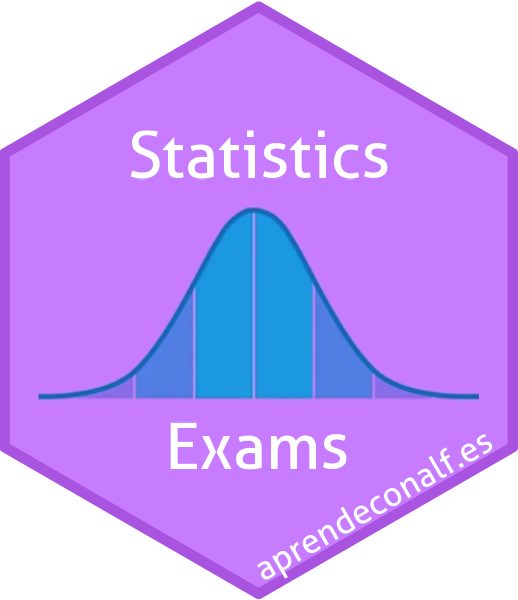
\includegraphics[width=0.4\textwidth]{img/logos/sticker.png}
\end{center}

\vfill

\begin{flushleft}
\begin{tabular}{ll}

\includegraphics[width=0.1\textwidth]{img/logos/aprendeconalf.png} & \parbox[b]{5cm}{\Large\textsf{Alfredo
Sánchez
Alberca}\\ \textsf{asalber@ceu.es} \\ \textsf{https://aprendeconalf.es}}
\end{tabular}
\end{flushleft}
\end{titlepage}\ifdefined\Shaded\renewenvironment{Shaded}{\begin{tcolorbox}[breakable, interior hidden, sharp corners, frame hidden, enhanced, borderline west={3pt}{0pt}{shadecolor}, boxrule=0pt]}{\end{tcolorbox}}\fi

\renewcommand*\contentsname{Table of contents}
{
\hypersetup{linkcolor=}
\setcounter{tocdepth}{2}
\tableofcontents
}
\bookmarksetup{startatroot}

\hypertarget{preface}{%
\chapter*{Preface}\label{preface}}
\addcontentsline{toc}{chapter}{Preface}

\markboth{Preface}{Preface}

Statistics exam collection of the Physiotherapy degree.

\bookmarksetup{startatroot}

\hypertarget{descriptive-statistics-and-regression-exam-20180531}{%
\chapter{Descriptive Statistics and Regression exam
(2018/05/31)}\label{descriptive-statistics-and-regression-exam-20180531}}

\leavevmode\vadjust pre{\hypertarget{exr-1}{}}%
\begin{exercise}[]\label{exr-1}

~

The ages of a sample of patients of a physical therapy clinic are:

\begin{table}
\centering
\begin{tabular}{r|r|r|r|r|r|r|r|r|r|r|r|r}
\hline
25 & 30 & 44 & 44 & 51 & 51 & 53 & 56 & 57 & 58 & 58 & 58 & 59\\
\hline
59 & 61 & 63 & 63 & 63 & 66 & 68 & 70 & 71 & 72 & 74 & 82 & 85\\
\hline
\end{tabular}
\end{table}

\begin{enumerate}
\def\labelenumi{\alph{enumi}.}
\item
  Compute the quartiles.
\item
  Draw the box plot and identify outliers (do not group data into
  intervals).
\item
  Split the sample into two groups, patients younger and older than 65.
  In which group is the mean more representative. Justify the answer.
\item
  Which distribution is less symmetric, the one of patients younger than
  65 or the one of patients older?
\item
  Which age is relatively smaller with respect to its group, 50 years in
  the group of patients younger than 65 or 72 years in the group of
  patients older than 65?
\end{enumerate}

Use the following sums for the computations.\\
Younger than 65: \(\sum x_i=953\) years, \(\sum x_i^2=52475\)
years\(^2\), \(\sum (x_i-\bar x)^3=-30846.51\) years\(^3\) and
\(\sum (x_i-\bar x)^4=939658.83\) years\(^4\).\\
Older than 65: \(\sum x_i=588\) years, \(\sum x_i^2=43530\) years\(^2\),
\(\sum (x_i-\bar x)^3=1485\) years\(^3\) and
\(\sum (x_i-\bar x)^4=26983.5\) years\(^4\).

\end{exercise}

\begin{tcolorbox}[enhanced jigsaw, left=2mm, leftrule=.75mm, opacitybacktitle=0.6, colframe=quarto-callout-tip-color-frame, title=\textcolor{quarto-callout-tip-color}{\faLightbulb}\hspace{0.5em}{Tip}, opacityback=0, breakable, bottomtitle=1mm, titlerule=0mm, colback=white, toptitle=1mm, coltitle=black, bottomrule=.15mm, toprule=.15mm, arc=.35mm, rightrule=.15mm, colbacktitle=quarto-callout-tip-color!10!white]

\begin{enumerate}
\def\labelenumi{\arabic{enumi}.}
\tightlist
\item
  \(Q_1=53\) years, \(Q_2=59\) years and \(Q_3=68\) years.
\item
  There are 2 outliers: 25, 30.
\end{enumerate}

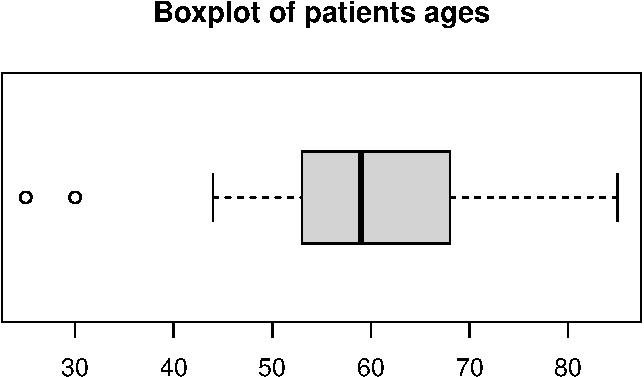
\includegraphics{./img/exam-2018-05-31/boxplot-ages-1.pdf}

\begin{enumerate}
\def\labelenumi{\arabic{enumi}.}
\setcounter{enumi}{1}
\tightlist
\item
  Let \(x\) be the age in patients younger than 65 and \(y\) the age in
  patients older than 65.\\
  \(\bar x=52.9444\) years, \(s_x^2=112.1636\) years\(^2\),
  \(s_x=10.5907\) years and \(cv_x=0.2\).\\
  \(\bar y=73.5\) years, \(s_y^2=39\) years\(^2\), \(s_y=6.245\) years
  and \(cv_y=0.085\).\\
  The mean is more representative in patients older than 65 since the
  coefficient of variation is smaller.
\item
  \(g_{1x}=-1.4426\) and \(g_{1y}=0.7621\), thus the distribution of
  ages of people younger than 65 is less symmetric.
\item
  The standard scores are \(z_x(50)=-0.278\) and \(z_y(72)=-0.2402\),
  thus 50 years is relative smaller in the group of people younger than
  65.
\end{enumerate}

\end{tcolorbox}

\leavevmode\vadjust pre{\hypertarget{exr-2}{}}%
\begin{exercise}[]\label{exr-2}

~

The table below shows the number of injuries of several teams during a
league and the average warm-up time of its players.

\begin{table}
\centering
\begin{tabular}{l|r|r|r|r|r|r|r|r|r|r}
\hline
Warm-up time & 15 & 35 & 22 & 28 & 21 & 18 & 25 & 30 & 23 & 20\\
\hline
Injuries & 42 & 2 & 16 & 6 & 17 & 29 & 10 & 3 & 12 & 20\\
\hline
\end{tabular}
\end{table}

\begin{enumerate}
\def\labelenumi{\alph{enumi}.}
\item
  Draw the scatter plot.
\item
  Which regression model is more suitable to predict the number of
  injuries as a function of the warm-up time, the logarithmic or the
  exponential? Use that regression model to predict the expected number
  of injuries for a team whose players warm-up 20 minutes a day.
\item
  Which regression model is more suitable to predict the warm-up time as
  a function of the number of injuries, the logarithmic or the
  exponential? Use that regression model to predict the warm-up time
  required to have no more than 10 injuries in a league.
\item
  Are these predictions reliable? Which one is more reliable?
\end{enumerate}

Use the following sums for the computations (\(X\) warm-up time and
\(Y\) number of injuries):\\
\(\sum x_i=237\), \(\sum \log(x_i)=31.3728\), \(\sum y_j=157\),
\(\sum \log(y_j)=24.0775\),\\
\(\sum x_i^2=5937\), \(\sum \log(x_i)^2=98.9906\), \(\sum y_j^2=3843\),
\(\sum \log(y_j)^2=66.3721\),\\
\(\sum x_iy_j=3115\), \(\sum x_i\log(y_j)=519.1907\),
\(\sum \log(x_i)y_j=465.8093\), \(\sum \log(x_i)\log(y_j)=73.3995\).

\end{exercise}

\begin{tcolorbox}[enhanced jigsaw, left=2mm, leftrule=.75mm, opacitybacktitle=0.6, colframe=quarto-callout-tip-color-frame, title=\textcolor{quarto-callout-tip-color}{\faLightbulb}\hspace{0.5em}{Solution}, opacityback=0, breakable, bottomtitle=1mm, titlerule=0mm, colback=white, toptitle=1mm, coltitle=black, bottomrule=.15mm, toprule=.15mm, arc=.35mm, rightrule=.15mm, colbacktitle=quarto-callout-tip-color!10!white]

\begin{enumerate}
\def\labelenumi{\alph{enumi}.}
\tightlist
\item
\end{enumerate}

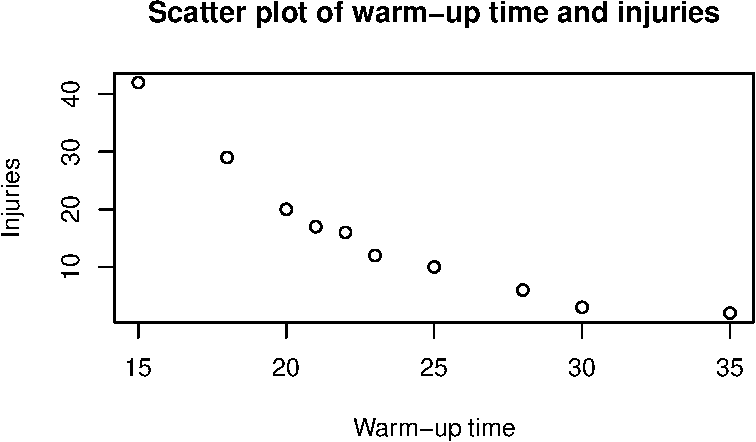
\includegraphics{./img/exam2018-05-31/scatterplot-injuries-warm-up-1.pdf}

\begin{enumerate}
\def\labelenumi{\alph{enumi}.}
\item
  \(\bar x=23.7\) min, \(s_x^2=32.01\) min\(^2\).\\
  \(\overline{\log(x)}=3.1373\) log(min), \(s_{\log(x)}^2=0.0565\)
  log(min)\(^2\).\\
  \(\bar y=15.7\) injuries, \(s_y^2=137.81\) injuries\(^2\).\\
  \(\overline{\log(y)}=2.4078\) log(injuries), \(s_{\log(y)}^2=0.8399\)
  log(injuries)\(^2\).\\
  \(s_{x\log(y)}=-5.1446\), \(s_{\log(x)y}=-2.6744\)\\
  Exponential determination coefficient: \(r^2=0.9844\)\\
  Logarithmic determination coefficient: \(r^2=0.9185\)\\
  So the exponential regression model es better to predict the number of
  injuries as a function of the warm-up time.\\
  Exponential regression model: \(y=e^{6.2168+-0.1607x}\).\\
  Prediction: \(y(20)=20.1341\) injuries.
\item
  The logarithmic model is better to predict the warm-up time as a
  function of the number or injuries.\\
  Logarithmic regression model: \(x=164.1851+-47.3292\log(y)\).\\
  Prediction: \(x(10)=55.2056112\) min.
\item
  Both predictions are very reliable since de deternation coefficient is
  very high but the last one is a little less reliable as it is for a
  value further from the data range.
\end{enumerate}

\end{tcolorbox}

\bookmarksetup{startatroot}

\hypertarget{descriptive-statistics-and-regression-exam-20230323}{%
\chapter{Descriptive Statistics and Regression exam
(2023/03/23)}\label{descriptive-statistics-and-regression-exam-20230323}}

\leavevmode\vadjust pre{\hypertarget{exr-1}{}}%
\begin{exercise}[]\label{exr-1}

~

The chart below shows the percentage of grades in a Statistic course
with 60 students.

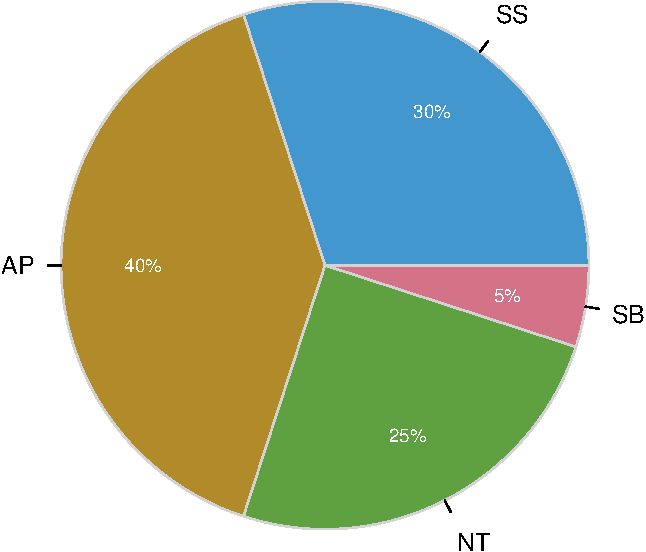
\includegraphics{./img/exam-2023-03-23/pie-chart-scores-1.pdf}

\begin{enumerate}
\def\labelenumi{\alph{enumi}.}
\tightlist
\item
  Plot the ogive of the score, assuming the following correspondence
  between grades and scores
\end{enumerate}

\[
\begin{array}{lc}
  \mbox{Grade} & \mbox{Score}\\
  \mbox{SS} & [0, 5)\\
  \mbox{AP} & [5, 7)\\
  \mbox{NT} & [7,9)\\
  \mbox{SB} & [9,10]
\end{array}
\]

\begin{enumerate}
\def\labelenumi{\alph{enumi}.}
\item
  Compute the median and interpret it.
\item
  How many students got a score greater than 8?
\item
  Study the dispersion of the distribution.
\item
  Study the skewness of the distribution. Is it normal?
\item
  If we apply the transformation \(y=10x+5\) to the scores, how changes
  the representativeness of the mean. And the skewness?
\end{enumerate}

Use the following sums for the computations (\(X\) = Score):\\
\(\sum x_in_i=337.5\), \(\sum x_i^2n_i=2207.25\),
\(\sum (x_i-\bar x)^3n_i=-172.55\) and
\(\sum (x_i-\bar x)^4n_i=2870.75\).

\end{exercise}

\begin{tcolorbox}[enhanced jigsaw, left=2mm, leftrule=.75mm, opacitybacktitle=0.6, colframe=quarto-callout-tip-color-frame, title=\textcolor{quarto-callout-tip-color}{\faLightbulb}\hspace{0.5em}{Tip}, opacityback=0, breakable, bottomtitle=1mm, titlerule=0mm, colback=white, toptitle=1mm, coltitle=black, bottomrule=.15mm, toprule=.15mm, arc=.35mm, rightrule=.15mm, colbacktitle=quarto-callout-tip-color!10!white]

\begin{enumerate}
\def\labelenumi{\alph{enumi}.}
\tightlist
\item
  Ogive
\end{enumerate}

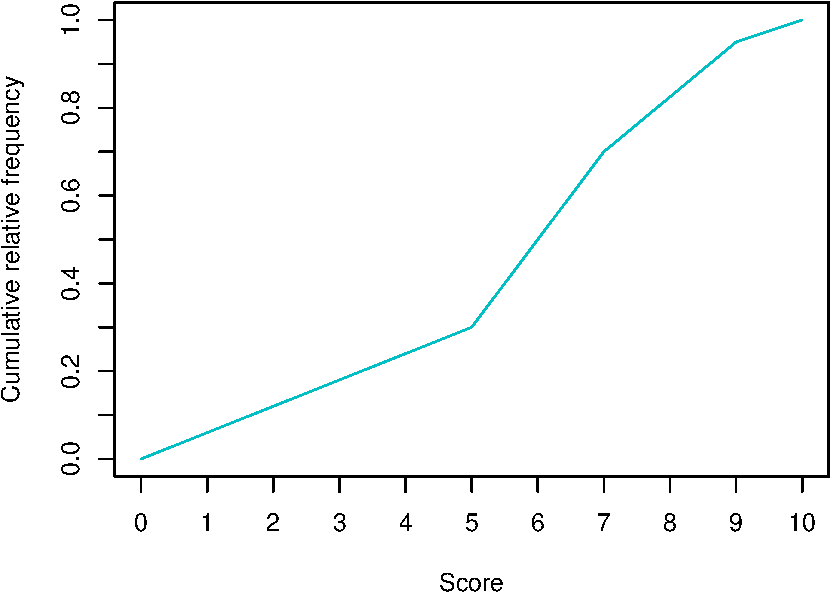
\includegraphics{./img/exam-2023-03-23/ogive-scores-1.pdf}

\begin{enumerate}
\def\labelenumi{\alph{enumi}.}
\setcounter{enumi}{1}
\item
  \(Me = 6\) points.
\item
  \(N(8) = 49.5\) students.
\item
  \(\bar x = 5.625\) points, \(s_x^2=5.1469\) points\(^2\),
  \(s_x=2.2687\) points and \(cv_x=0.4033\). Thus, there is a moderate
  dispersion with respect to the mean.
\item
  \(g_1 = -0.2463\) and therefore the distribution is a little bit left
  skewed.
\item
  \(\bar y = 61.25\) points, \(s_y^2=514.6875\) points\(^2\),
  \(s_y=22.6867\) points and \(cv_y=0.3704\). As \(cv_y < cv_x\) the
  representativeness of the mean increases. As the slope of the linear
  transformation is positive, the skewness does not change.
\end{enumerate}

\end{tcolorbox}

\leavevmode\vadjust pre{\hypertarget{exr-2}{}}%
\begin{exercise}[]\label{exr-2}

~

A study tries to determine if there is a relation between the gestation
time (in weeks) and the age of the mother (in years). A sample of 40
mothers was taken and the sums below summarize the results (\(X\)=Age
and \(Y\)=Gestation time):

\(\sum x_i=1262\) years, \(\sum \log(x_i)=137.0078\) log(years),
\(\sum y_j=1583.6\) weeks, \(\sum \log(y_j)=147.1305\) log(weeks),\\
\(\sum x_i^2=41862\) years\(^2\), \(\sum \log(x_i)^2=471.4222\)
log(years)\(^2\), \(\sum y_j^2=62734.685\) weeks\(^2\),
\(\sum \log(y_j)^2=541.2096\) log(weeks)\(^2\),\\
\(\sum x_iy_j=50116.7\) years\(\cdot\)weeks,
\(\sum x_i\log(y_j)=4645.8\) years\(\cdot\)log(weeks),
\(\sum \log(x_i)y_j=5428.9192\) log(years)\(\cdot\)weeks,
\(\sum \log(x_i)\log(y_j)=504.0696\) log(years)\(\cdot\)log(weeks).

\begin{enumerate}
\def\labelenumi{\alph{enumi}.}
\item
  Which regression models, linear, exponential or logarithmic, explains
  better the relation between the age and the gestation time?
\item
  Use the best model to predict the gestation time for a mother 45 years
  old. Is this prediction reliable?
\item
  According to the linear model, how much increases or decreases the
  gestation time for every year of the mother?
\end{enumerate}

\end{exercise}

\begin{tcolorbox}[enhanced jigsaw, left=2mm, leftrule=.75mm, opacitybacktitle=0.6, colframe=quarto-callout-tip-color-frame, title=\textcolor{quarto-callout-tip-color}{\faLightbulb}\hspace{0.5em}{Solution}, opacityback=0, breakable, bottomtitle=1mm, titlerule=0mm, colback=white, toptitle=1mm, coltitle=black, bottomrule=.15mm, toprule=.15mm, arc=.35mm, rightrule=.15mm, colbacktitle=quarto-callout-tip-color!10!white]

\begin{enumerate}
\def\labelenumi{\alph{enumi}.}
\item
  Linear model: \(\overline{x}=31.55\) years, \(s_x^2=51.1475\)
  years\(^2\).\\
  \(\bar y=39.59\) weeks, \(s_y^2=0.999\) weeks\(^2\).\\
  \(s_{xy}=3.853\) years\(\cdot\)weeks.\\
  \(r^2 = 0.2905\).

  Exponential model: \(\overline{\ln(y)} = 3.6783\) ln(weeks),
  \(s_{\ln(y)}^2 = 0.0006\) ln(weeks)\(^2\)\\
  \(s_{x\ln(y)} = 0.0958\) years\(\cdot\ln\)(weeks).\\
  \(r^2 = 0.2882\).

  Logarithmic model: \(\overline{\ln(x)} = 3.4252\) ln(years),
  \(s_{\ln(x)}^2 = 0.0536\) ln(years)\(^2\)\\
  \(s_{\ln(x)y} = 0.1195\) ln(years)weeks.\\
  \(r^2 = 0.2668\).

  As the linear coefficient of determination is greater, the linear
  model explains better the relation between de gestation time and the
  age of the mother.
\item
  Linear regression model of \(Y\) on \(X\):
  \(y = 37.2133 + 0.0753 x\).\\
  Predictions: \(y(45) = 40.6032\) weeks.\\
  The predictions are not reliable because the coefficient of
  determination is pretty low.
\item
  Regression coefficient of \(Y\) on \(X\): \(b_{yx} = 0.0753\)
  weeks/year. The gestation time increases \(0.0753\) weeks per year.
\end{enumerate}

\end{tcolorbox}



\end{document}
